% Repositioning.tex
% Submitted 29/11/2016
% Interim decision 27/03/2017
% resubmitted 9/06/2017
% resubmitted (again) 10/09/2017
% The Journal of Biomedical Informatics 

%\documentclass[preprint,review,12pt]{elsarticle} 
\documentclass[preprint,11pt]{elsarticle} 
\usepackage{amssymb}
\usepackage{epsf}
\usepackage{graphicx}
\usepackage{epstopdf}
\usepackage{natbib} 
\usepackage{mathtools}
\usepackage[margin=1in]{geometry}
\usepackage{epstopdf}% To incorporate .eps illustrations using PDFLaTeX, etc.
%\usepackage{subfigure}% Support for small, `sub' figures and tables
\usepackage[table]{xcolor} 
\usepackage{graphicx}% http://ctan.org/pkg/graphicx
\usepackage{array}% http://ctan.org/pkg/array
\usepackage{amsmath}
\usepackage{algorithmicx}
\usepackage{algorithm}
\usepackage{algpseudocode}
\usepackage{caption}
\usepackage{subcaption}
\usepackage{verbatim}

\begin{document} 
\begin{frontmatter}
\title{Identifying drug candidates for repositioning through side-effect similarity and integration of supporting knowledge using computational intelligence}
\author{Ken McGarry, Yitka Graham, Sharon McDonald and Anuam Rashid}
\address{School of Pharmacy and Pharmaceutical Sciences, Faculty of Health Sciences and Wellbeing,\\University of Sunderland, UK}

\begin{abstract}
The objective of drug repositioning is to apply existing drugs to different diseases or medical conditions than the original target, and thus alleviate to a certain extent the time and cost expended in drug development. The area of drug repositioning is a suitable application area for computational intelligence because numerous online databases containing technical information on drug targets, protein interactions, side-effects and biological knowledge are currently available. We propose that drugs with similar side-effects are potential candidates for use elsewhere, the supposition is that similar side-effects may be caused by drugs targeting similar proteins.  We evaluate the shared side effects from the eight Alzheimer drugs that try to slow down the degeneration or treat the symptoms. We identified sixty-seven candidate drugs based on a side-effect commonality of at least 50\%, the most similar 25 drugs on the list were further investigated in depth for their suitability to be repositioned. We checked the literature and several of the 25 drugs appear to have been trialled for Alzheimer's disease with varying degrees of success. Thus verifying the accuracy of our system, therefore, given sufficient side-effect similarity between conventional treatment drugs and those drugs that appear to be interacting with similar targets it is possible to identify new candidate drugs that may be further evaluated. We also compare our technique with several competing systems found in the literature.
\end{abstract}

\begin{keyword}
side-effects; graph theory; pattern matching; protein targets;
\end{keyword}

\end{frontmatter}

\section{Introduction}
In this paper we explore how adverse drug side-effects, stored in a large database can be used to identify potential candidates for drug repositioning for Alzheimer's disease. Drug re-purposing or repositioning involves using existing pharmaceutical products on novel targets, the advantages are many; off-the-shelf drugs have undergone extensive testing and their toxicological properties are well known, therefore the costs are greatly reduced and also time to product delivery \cite{Liu2014}. Thus it is more economical to re-purpose an existing drug than develop one from scratch \cite{Dudley2011}.  Difficulties in drug development arise because diseases are often complex with multi-factorial components such as interactions between genes, proteins and the environment \cite{Barrenas2009}. Furthermore, drugs that are highly selective in terms of their targets are very rare. The usual situation is that a drug will target the proteins involved in the defective biological process but also interact (side-effects) to a lessor or greater extent with off-target proteins \cite{Yang2014,Bisgin2012}. This feature can be used to search for  drugs with similar side-effects that might target the defective biological functions more effectively than conventional drugs.

%%%%%%% Figure %%%%%%%%%%%%%%%%
\begin{figure*}[h]
%\epsfysize=4.0cm \leavevmode
  \begin{center}
	 \includegraphics[width=14cm,height=10cm]{/LaTex/Reposition/workflow.pdf} % OK
  \end{center}
\special{center} \caption{Overview of system operation, showing database sources, data flow and statistical analysis}
\label{system}
\end{figure*}
%%%%%%%%%%%%%%%%%%%%%%%%%%%

Recently, there has been a great deal of interest in discovering potential drugs that show potential for repositioning for Alzheimer's disease \cite{Corbett2012}. Alzheimer's is a degenerative disease in which both genetic and non-genetic factors can contribute to a progressive decline in the individual and is likely to affect 65 million adults world-wide by 2030 \cite{Bandyopadhyay2014}.  There are several proteins implicated with the onset of the disease, the Amyloid-$\beta$ Precursor Protein (APP) is of major interest as it forms plaques and is seen a contributing factor in dementia. However, Alzheimer’s is a complex disease due to having many genes and proteins with a high level of interactivity between them and drugs that target individual proteins may not be an optimum solution \cite{Re2013,Oh2014}. 
 
Our objective  is to identify drug repurposing candidates for Alzheimer's disease, the approach taken in this paper is to view the problem as one of identifying and assessing side-effects in known drugs \cite{McGarry2015a,Kuhn2010}.  The system we developed is shown in figure \ref{system}, we obtain and examine the side-effects of the eight most common Alzheimer's (Donepezil, Galantamine, Rivastigmine, Citalpram, Risperidone, Memanatine, Escitalopram and Aripiprazole) drugs found in the SIDER4 database. The drugs were compared against their chemical properties, on-targets and off-targets which provided further information necessary to prune down the list of potential candidate drugs. The other databases include the gene ontology and the disease ontology, these provide expert level descriptions of biological functions, structures and the genes involved in the pathways targeted by the drugs.  Furthermore, they provide an indication of similarity between diseases and links between shared genes and pathways. In this paper we extend previous work by incorporating chemical structure information from CHeMbL and also knowledge from the two main biological ontologies (gene and disease ontologies) to enhance biological understanding. Furthermore, we extend the analysis of the side-effect types in terms of severity of effect and effect type.

\subsection{Related work}
The PREDICT system developed by Gottleib et al  tackles the issue from the viewpoint of large scale drug indications for personalised medicine \cite{Gottlieb2011}. The system analyses both approved and novel drugs, basing its recommendations on the observation that similar drugs affect similar diseases and they devise appropriate distance measures to implement this. PREDICT is able to build a model of disease specific signatures that can be used assist the drug targeting process, a comparison with PREDICT and our system is made in the results section.

The connectivity map (CMAP) of Cheng et al was developed by compiling the data available from Affymetrix genechips taken from 13,000 human samples (9,000 diseased and 3,400 healthy individuals) \cite{Cheng2014}. These were mapped against 152 drug profiles and 145 disease gene signatures, this was achieved by using the {\it eXtreme Sum} (XSum) scoring algorithm. The authors concluded that although they could identify drug-interaction pairs they admitted the CMAP method required better validation data as some diseases had worse than random performance.

The system developed by Chiang and Butte uses a guilt by association (GBA) method which involves mapping the diseases to one logical set and mapping the drugs to another set, the degree of overlap between the two sets was determined systematically  \cite{Chiang2009}. The authors claim to have produced 57,000 novel drug uses of which only a small number could be verified and the false positive rate appears rather high. 

The SLAMS method proposed by Zhang of the IBM Research Center, integrates several sources of data such as chemical structure and protein targets, chemical data is integrated through the creation of binary fingerprints \cite{Zhang2013,Zhang2014}. The SLAMS algorithm uses several novel features for improving the accuracy such as the ability to impute missing values of side-effects profiles which are then incorporated with the predicted profiles for improved side-effect knowledge. Furthermore, several methods such as ROC, AUC and F-scores are used to evaluate the prediction accuracy, 10-fold cross-validation is used is used to enhance the accuracy of their models. Further work by this group (Wang) in drug repositioning concentrated on predicting drug side-effects based on drug therapeutic indications and vice-versa using a variety of predictor variables \cite{FWang2014}. We found this work to be particularly illuminating as it is the basis for our own research and we compare our results with Zhang's. 

The work of Guney provides insights into why drug similarity does not always account for identifying useful drugs for repositioning \cite{Guney2016a,Guney2017}. Guney provides a deep evaluation of many diseases and drug pairs to create a complex network of interactions that reveals how diseases and their drugs are clustered into neighborhoods of proximity. They used the concept of proximity to develop a better understanding of how disease  modules operate with their associated target proteins and drug mode of action. Guney also demonstrated how knowledge of  proximity can be used to predict the therapeutic action and side-effects of known drugs.

The drug-target-disease network by Daminelli \cite{Daminelli2012} was created by integrating disease-to-chemical associations which were later datamined for combinations of network motifs. The bi-cliques produced appear to have a high false positive rate through using only the complex networks structure. However, the authors did an analysis to reveal the most promiscuous drugs in terms of multiple targets and diseases which will assist those seeking drugs to repurpose in those areas.
 
The complex network analysis performed by Wang {\it et al} used a heterogeneous graph based inference (HGBI) method which involved using 5080 diseases, 1409 drugs and 3989 targets \cite{Wang2014}. A triple layer network model was built using this data,  In addition to the normal process of selecting candidate drugs using known treatments, Wang also applies his method to diseases with no known drugs, the system was able to perform well by ranking drugs that have received attention in the clinical trials literature. How the HGBI system  will cope with the addition of further layers and different datasets remains to be seen but the authors intend to verify their work with wetlab experimental work. We compare our results with Wang's in the results section.

The work of Zhang {\it et al} is notable because they generate a list of proteins to be targeted by specific drugs using an omics based approach \cite{Zhang2016}. They used OMIM database to provide information on SNP and genomic details and generated a candidate list of 524 Alzheimer's disease implicated proteins. Some were known from the literature and some were speculative. A number of targets were implicated for treating acute myelogenous leukemia (Gemtuzumab, ozogamicin, Vadastuximab talirine and Lintuzumab). Refining their search they pruned the candidates down to 18 protein targets linked to 75 existing drugs, including seven  drugs inhibiting Alzheimer's targets.

A different approach was taken by Luo, whereby a specific family of proteins cyclooxygenase (COX) inhibitors were targeted \cite{Luo2016,Luo2017}. These are useful in preventing inflammatory diseases and have wide application in pain reduction and are a type of non-steroidal anti-inflammatory drug (NSAID). Various techniques including dimensionality reduction were used to  manage the large network of 12,000 nodes and nearly 2 million connections. The initial analysis of the network was followed up by molecular modeling software to test out the docking abilities of their discovered candidate targets. The most promising ones were wetlab tested using mice kidney and macrophhage assays, for the drugs Telmisartin, Chlorproamide and Alendronate. All three drugs appear to be useful binders to COX1 and COX2 inhibitors, thus validating their method. Other researchers has concentrated on applying various combinations of methods described above \cite{Ye2014, XWang2013, Liu2016, TLiu2015,ChaoWu2013}.

The novel aspects of our work include a strong level of biological knowledge  through the use of pathway and biological information  integration. This provides a level of understanding lacking in most of the existing methods, it enables the users to relate drugs to their side-effects and on/off protein targets. The disparate sources of data are integrated through the use of a modified Jaccard coefficient We verify our work through the analysis of our top scoring drugs against evidence from the drug repurposing literature and compare our method against several of the most similar computational techniques. 

The remainder of this paper is structured as follows; section two describes the methods, discussing the data used and the assumptions we have made, the overall system architecture is described along with the computational techniques used to search, pre-process and model the data; section three outlines the  results of analyzing the types of side-effects and protein on-targets of the Alzheimer disease state and the protein off-targets that are shared by the candidate drugs; section four presents the discussion; finally section five draws out the conclusions and possible areas for future work.


\section{Methods}
In the following discussions, reference should be made to figure \ref{process} for clarification of dataflow and processing.

\subsection{Data bases and sources of information}
The initial starting point for using our system is to obtain the UMLS code for the disease of interest. This code is used to interrogate the DrugBank database to provide a list of known, conventional treatments.  Drugbank contains the majority of drugs that are currently prescribed, or have been withdrawn or are at the clinical trial stage. This resource is widely used by those developing drugs, chemists, pharmacologists and others involved in pharmaceutics research \cite{Law2014}. Every drug is listed with its main targets, known off-targets along with chemical structure and other important characteristics. 

Having obtained a list of conventional  drugs used to treat the disease of interest, the SIDER4 database is  accessed to give a list of side-effects for each drug. SIDER4, an important repository of hundreds of drugs and thousands of their known side-effects on humans \cite{Kuhn2013}. This freely available database contains more than 1,430 drugs and 58,880 side effects. The information on the drugs is collected, from the national registries and charity organisations \cite{Kuhn2010}. In addition to side-effects for the 1,430 drugs SIDER4 also has information on the frequency of their relative occurrence in patients. It should be noted that SIDER4 contains many more side-effects per drug  than would normally appear in the packet-insert that is included in every drug prescription.  

We removed from SIDER4, 10\% of the most common side-effects that occur with most drugs such as Nausea, Dermatitis, Rash, Vomiting, Headache, Dizziness etc as per the work of Atias \cite{Atias2011}. In total, 573 side-effect types were removed. Further preprocessing replaced lengthy drug/compound names with their drugbank identifiers. For example (10ALPHA,13ALPHA,14BETA,17ALPHA)-17-HYDROXYANDROST-4-EN-3-ONE becomes DB07768.

%%%%%%% Figure %%%%%%%%%%%%%%%%
\begin{figure*}[h]
%\epsfysize=4.0cm \leavevmode
  \begin{center}
	 \includegraphics[width=12cm,height=10cm]{/LaTex/Reposition/process.pdf} % OK
  \end{center}
\special{center} \caption{Detailed step by step process diagram}
\label{process}
\end{figure*}
%%%%%%%%%%%%%%%%%%%%%%%%%%%

Our basic proposition is that shared side-effects between the drugs used to treat a disease can be combined into a search pattern to interrogate the SIDER4 database again to identify candidate drugs causing similar side-effects. The assumption is that these drugs are targeting similar biochemical pathways (inadvertently) and therefore may be candidates for re-purposing to the original disease. The side-effects pertaining to the nine drugs commonly used to treat Alzheimer's Disease (AD),  such as Donepezil, Galantamine and Rivastigmine were obtained from the SIDER4 database.

Once a list of new, candidate drugs has been generated and sorted according to their percentage side-effect similarity, other databases can be interrogated for chemical structure, protein targets and biological pathways relating to these drugs. These results are further enhanced by enrichment from gene ontology and disease ontology for biological plausibility.

%Referring to table \ref{S4} the first column is the entry for the Pubchem compound identifier, the second is the %identifier as described in the STITCH database, the third column is the UMLS concept identifier for the side-effect as %it was found on the package label, the fourth is the common drug name, the fifth is the side effect name as it %appears in the package leaflet, the sixth column is the  MedDRA concept type (LLT = lowest level term, PT = %preferred term), the seventh column refers to UMLS concept identifier for MedDRA side-effect term, finally the %eighth column contains the MedDRA side effect name.

% latex table generated in R 3.2.2 by xtable 1.8-2 package
% Thu Jul 07 14:27:01 2016
%\begin{table}[h]
%\scriptsize
%\centering \caption{Internal structure of the SIDER4 database displaying 20 side-effects for the  drug Tramadol}
%\begin{tabular}{llllllll} \hline
% compound  & STITCH & UMLS  & drug  & side effect  & MedDRA & U/MeDRA & MedDRA side effect \\  \hline
%100005523 & 33741 & C0426732 & tramadol & enlarged prostate & LLT & C0426732 & Enlarged prostate \\ 
% 100005523 & 33741 & C0426732 & tramadol & enlarged prostate & PT & C0847978 & Prostatomegaly \\ 
%100005523 & 33741 & C0003486 & tramadol & aortic aneurysm & LLT & C0003486 & Aortic aneurysm \\ 
%100005523 & 33741 & C0003486 & tramadol & aortic aneurysm & PT & C0003486 & Aortic aneurysm \\ 
% 100005523 & 33741 & C0392386 & tramadol & decreased platelet & LLT & C0392386 & Platelet count decreased \\ 
%100005523 & 33741 & C0392386 & tramadol & decreased platelet & PT & C0392386 & Platelet count decreased \\ 
 %100005523 & 33741 & C0027651 & tramadol & tumor & LLT & C0027651 & Neoplasm \\ 
 %100005523 & 33741 & C0027651 & tramadol & tumor & PT & C0027651 & Neoplasm \\ 
%100005523 & 33741 & C0024031 & tramadol & low back pain & LLT & C0024031 & Low back pain \\ 
%100005523 & 33741 & C0024031 & tramadol & low back pain & PT & C0004604 & Back pain \\ 
%100005523 & 33741 & C0009763 & tramadol & conjunctivitis & LLT & C0009763 & Conjunctivitis \\ 
 %  \hline
%   \label{S4}
%\end{tabular}
%\end{table}
%\normalsize

The chemical structure of the candidate drugs was downloaded from CHemBL, this database contains chemical compounds represented as text data called the SMILES (Simplified Molecular Input Line Entry System) format \cite{Weininger1988}. We created a series of fingerprints for each drug based on atom-pair arrangements of 2048 bits in size. We consider the chemical structure of the candidate drugs useful information to assess their suitability for repositioning.

The candidate drugs have known on-target and off-target proteins, this knowledge is augmented by accessing protein-to-protein interactions and drug to protein interactions found in the STITCH and STRING databases \cite{Kuhn2012}. The STRING database  makes use of over six million known protein-to-protein interactions discovered by text mining and annotation by human experts. Additionally,  a further 30,000 associations are predicted based on similar protein characteristics using predictive data mining. The STITCH database contains protein to chemical mappings and augments the information held in Drugbank which may not contain all the potential drug to protein interactions. 

The Reactome database is accessed to provide indications of which biological pathways are involved with the on-target and off-target protein interactions affected by the candidate drugs \cite{Yu2015c}. Deeper insights can be gained into the biological functions by allowing users of the system to relate side-effects to drugs and then to the pathways. Individual proteins must not be regarded in isolation but seen as a system of interacting components. The associated pathways are incorporated into the overall drug ranking measure.


\subsection{Searching for side-effect similarity}
The work described in this paper extends the complex network and pattern matching algorithms previously developed by the authors \cite{McGarry2015a, McGarry2015b,McGarry2016a} to include a novel data integration method that  assesses the candidate drugs, their chemical characteristics, associated proteins and biological pathways as described in section \ref{integration}. 

\begin{algorithm}
\caption{Identification of drugs with similar side-effects}\label{alg1}
\begin{algorithmic}[1]
\scriptsize
\Procedure{SearchSideEffects}{$DRUGBANK,SIDER4,UMLS$}\Comment{Databases used}
   \State{\textit{\bf do initialize}}
   \State $umls \gets \mbox {get UMLS code for disease}$\Comment{e.g. C0002395 for Alzheimer's}
   \State $SE_{threshold} = 3$\Comment{A drug must have 3 or more side-effects to be useful}
   \State $drugcount =0$\Comment{setup for N drugs for the disease }
   \State $SIM_{cutoff} =$ 50\Comment{$>$ 50 percent similarity required}
    \State{\textit{\bf end initialize}}  
    \State{$DrugList \gets  DRUGBANK[umls]$}\Comment{Search DRUGBANK for drugs treating this disease}
    \State{$drugcount \gets length(DrugList)$}
   \For{\textit{$i \leq drugcount$}}
           \State \textit{$i_{se} \gets SIDER4[i]$}\Comment{For each drug get associated side-effects}
           \State \texttt{$se_{count}[i] \gets length(i_{se})$}\Comment{count side-effects}
            \If{$se_{count} [i] >$ \textit{$SE_{threshold}$}}
            \State \texttt{$DrugList[i] \gets DrugList[i]$}\Comment{Update DrugList with usable drugs}
            \State \texttt{$SE[i] \gets i_{se}$}\Comment{Save Drug side-effects}
            \EndIf
   \EndFor  
            \State{$JSE \in  SE[i]$}\Comment{Get Joint Side-Effects for Current drugs}
   		   \For{\textit{$j \leq DrugList[i]$}} 
   		   \State{$ReposList[j] \gets SIDER4 \subset JSE$}\Comment{Search SIDER4 for any new drug with these side-effects}
                   \State \textit{$Drug_{percentage}[j] \gets CalcPercentageSimilarity(ReposList[j])$  }\Comment{}
                   \If{$Drug_{percentage} [j] >$ \textit{$SIM_{cutoff}$}}
                   \State \texttt{$ReposList[j] \gets ReposList[j]$}\Comment{Create ReposList with candidate drugs}
                   \EndIf
                \EndFor
            \State{$Sort ReposList[j] descending order$}    
       \State \textbf{return} $ReposList, SE, SE_{common}$\Comment{Return drugs with $>$  50 percent similarity and their side-effects} 
\EndProcedure
\normalsize
\end{algorithmic}
\end{algorithm}

Referring to algorithm \ref{alg1}, lines 2-7 perform the initialization of key values: to obtain the UMLS code for the disease of interest, for the minimum number of side-effects for a viable search to be conducted (set at $\geq$ 3), the number of conventional drugs currently treating this disease is set to zero and finally a percentage value of side-effects similarity for a candidate drug to be considered useful (set at 50\%). 

Lines 8-9 obtain the drugs currently treating the disease of interest. Lines 10-17 ensure that each conventional drug is annotated with a list of more than three or more side-effects, if any drug has fewer than three side-effects it is discarded. The critical processing is performed by line 18 which creates a list of the side-effects common to all of the  conventional drugs. This list of common side-effects is used by lines 19-25 to search SIDER4 and return any candidate drug that has at least one side-effect in the search list. The new list of repositioned candidate drugs is sorted by lines 26-27, in descending order and only those with greater than 50\% similarity are returned from the function call.

Empirically, it was determined that conventional drugs with fewer than three side-effects are generally not useful as they tend to have either highly specific or overly common side-effects. They cannot provide a rich enough search pattern and these are pruned from the list of drugs. The common side-effects for the remaining conventional drugs are determined, this is used to search SIDER4 again for any candidate drug having at least one side-effect in common. 


\subsection{Graph theory}
We use graph theoretic methods to build networks of interacting proteins such as the drug on-targets and off-targets (where known). These networks provide various statistical measures describing the relationships between the interacting proteins and the candidate drugs, with some tentative indications of why a particular side-effect occurs.  We incorporate these statistical measures into the overall integration mechanism, which contributes in ranking the drugs in terms of usefulness for repositioning. 

Graph creation and inferencing is usually through matrix algebra, edge lists are converted into connectivity matrices, we can define a graph G = (V, E) where the nodes also called vertices V containing links called edges E. The links can be either directed, that is to say information implying direction or causality in the relationship is available in the sense that A causes B. Links can also be undirected, implying that we only know there is a relationship between the nodes but are unable to specify the sequence of events or perhaps this information is unnecessary. In our application, we determine the relevance of protein connectivity patterns using criteria from the graph theoretic centrality statistics, see equations 1-5 \cite{Freeman1979, Barabasi2004}.

We use a number graph based measures to evaluate the protein networks. %\verb|graybox| 
The closeness statistics provides a measure of how close each node is to every other node in the network. Some nodes may be more prominent than others due to their topology.
\begin{equation}\label{closeness}
     CC(v_i) =  \frac{N - 1}{\sum_{j} d(v_i,v_j)}
\end{equation}

The betweeness statistic calculates the extent that a node is located between pairs of other nodes in the network, such that a path between the other nodes has to go through that node.

\begin{equation}\label{betweenness}
     BC (v_k) =  \sum_{i} \sum_{j} \frac{p(v_i,v_j,v_k)}{p(v_i,v_j)}, i \neq j \neq k
\end{equation}

The clustering coefficient provides a measure of modularity of the network in terms of shared components.

\begin{equation}\label{clustercoeff}
     C_{i}  =  \frac{2\mid\{e_{jk} \}\mid}{k_{i}(k_{i} - 1)} : v_{j}, v_{k} \in N_{i}, e_{ij} \in E
\end{equation}

Where $V = v1, v2  ... vn$ define the $n$ vertices or nodes and $E$ the collection of edges or connections, where $e_{ij}$ indicates an edge (E) connecting vertices $v_i$, the term $v_j$ $k_i$ represents the vertex (V) neighbourhood. The neighbours $N$, for a given vertex (V) $v_i$, is its closely connected neighbours :

\begin{equation}\label{neighbour}
     N_{i}  =  \{v_{j}\}:e_{ij} \in E
\end{equation}

The in-degree and out-degree of each the vertices (in undirected graphs it is just overall degree) $k_i$  corresponds to the number of vertices in its near neighbourhood $| Ni |$.  Calculating the clustering coefficient $C_i$ for each vertex $v_i$ the ratio of links between the vertices within its near neighbourhood partitioned by the total  links that potentially could occur between them. Furthermore, graphs that are undirected have the characteristic that $e_{ij}$ and $e_{ji}$ are considered equivalent. 

\begin{equation}\label{edges}
    \frac{k_{i}(k_{i} - 1)}{2}
\end{equation}

A value of unity is returned when all vertices connected to $v_i$ are also linked to all other vertices
within the neighbourhood $n$, and returns zero when no vertex connected to $v_i$ links to all other vertices that connect to $v_i$.  
%\end{svgraybox}

\subsection{Gene ontology}
Gene ontology (GO) provides useful biological information and it is recognized as the {\it de facto} standard for gene product annotation. For our purposes, we produce a binary matrix of proteins annotated with the presence or absence of  terms. This enables an assessment to be made regarding the biological plausibility of the interacting proteins to observe the extent they actually cooperate in viable biological functions rather than random or spurious associations. For each protein associated with the candidate drugs enrichment was performed using gene ontology (GO), the enrichment is based on similarity measures using information content techniques. The content of which is calculated by taking the negative log probability of the terms $t$ appearing in the database. A number of measures can be used to rank semantic similarity, we used the {\it Wang} criterion as it reflects the biological plausibility better than other measures because of the way semantic similarity of the GO terms are calculated, using both the locations of the terms in the GO graph and their relations with their ancestor terms \cite{Wang2007}.

\begin{equation}
         Wang(A, B) = \frac{\displaystyle\sum_{t \in T_{A} \cap T_{B}}{S_{A}(t) + S_{B}(t)}}{SV(A) + SV(B)}
\label{goe}
\end{equation}

For the Wang equation, where $SA(t)$ represents the S-value of GO term $t$ related to term $A$ and $SB(t)$ is the S-value of GO term $t$ related to term $B$. 

\subsection{Drug chemical fingerprints}
The chemical data held in the large SDF file is used to create a unique fingerprint for each drug. We used the Tanimoto similarity coefficient was to compare the chemical structure of our 77 drugs based on pairwise binary fingerprints \cite{Chen2002}. The Tanimoto coefficient generally gives better results than other metrics. Equation \ref{tanimoto} shows the method of matching for the algebraic form.

\begin{equation}\label{tanimoto}
     S_{A,B}  =  \frac{\sum\limits_{i=1}^m n_{A,i} n_{B,i}}{\sum\limits_{i=1}^m  n_{A,i}^2+ \sum\limits_{i=1}^m n_{B,i}^2 - \sum\limits_{i=1}^m n_{A,i} n_{B,i}}  
\end{equation}

where: A is the number of unique fragments in the first compound and B is the number of unique fragments in the second compound; $ n_{A,i} $ is the shared amount of fragment  {\it i} in A; and $ n_{B,i} $ is the amount of fragment {\it i} in compound B.

Thus we would expect to see drugs with similar chemical structures to have similar properties and medicinal effects.

\subsection{Disease ontology}
We integrated information from the Disease Ontology (DO)   to annotate the drug targets and other proteins to obtain a deeper interpretation of the biological processes and structures \cite{Yu2010,Jiang2011,Schriml2012}. The DO database contains knowledge on 8,043 inherited, developmental and acquired human diseases. Through enrichment analysis, the R package  DOSim is able to explore the biological meaning of related genes in terms of structure, function and hierarchy. The concepts in DOSim are organized into a directed acyclic graph (DAG) similar to a tree structure, the concepts are linked by' is-a' relationships. The lower the term or concept is positioned in the hierarchy then the more specific the term is, higher-up terms describe higher level or more abstract concepts. In order to identify biological themes the Hypergeometric model is used to assess the frequency of those semantic terms
in a list and to determine whether the number of selected genes associated with disease is larger than expected than by chance alone.

\begin{equation}
        p = 1 - \displaystyle\sum_{i = 0}^{k-1}\frac{{M \choose i}{{N-M} \choose {n-i}}} {{N \choose n}}
\label{doe}
\end{equation}

Where $N$ is the total number of genes present in the distribution, $M$ is the number of genes within that distribution that are annotated (either through primary links or secondary links) to the node of interest, $n$ is the size of the list of genes of interest and $k$ is the number of genes within that list related to the node. 

\subsection{Data integration}\label{integration}
Individually, each method of data analysis  provides important information in a specific area. However, our systems strength comes from the integration of these disparate sources of  knowledge in a principled way. We use  a variation of the Jaccard similarity coefficient to integrate the many sources of heterogenous information into a coherent entity for decision making \cite{BenHur2002}.

\begin{eqnarray}
        Score  = \text{disease}_{ij} + \text{ontarget-proteins}_{ij} \text{+ off-target-proteins}_{ij} + \nonumber \\
        \text{pathways}_{ij} + \text{sideeffects}_{ij} + \text{chemicalsimilarity}_{ij} +\text{GO-DO-similarity}_{ij}
\label{integrate}
\end{eqnarray}

\begin{equation}
        \text{Score index}_{ij} = \frac{\vert F(D_{i}) \cap F(D_j)\vert} {\vert F(D_{i}) \cup F(D_j) \vert}\nonumber
\label{associndex}
\end{equation}

Where $F(D_j)$ are the features of interest, such as disease/symptom to treat, proteins, side-effects and chemical similarity shared between the candidate drugs $F(D_i)$. The candidates are then reevaluated using these scores and re-ranked according to their potential for repurposing.

\subsection{Hardware and software platform}
We implemented the system using the R language with the RStudio programming environment, on an Intel Xenon 64-bit CPU, using dual processors (3.2GHz) with six cores, and 128 GB of RAM. R is primarily a statistical data analysis package but is gaining popularity for various scientific programming applications and is very extendable using packages written by other researchers \cite{RUser}.  We used the following R packages: GOSim \cite{Yu2015}, DOSim \cite{Yu2010}, ChemmineR\cite{Cao2008}. Since it is an interpreted language, R is generally quite slow compared with a compiled language. However, we used the MicroSoft R Open system (https://mran.microsoft.com/) because it is optimized to take advantage of processor cores and the majority of its mathematics/matrix operations are rewritten in C++ to speed up operation. It is fully compatible with the oringinal CRAN version of R. Our R code and data files are freely available to all researchers on GitHub for download:\\ {\bf https://github.com/kenmcgarry/DrugSideEffects}


\section{Results}
Our first step is to obtain the UMLS code for our disease of interest (Alzheimer's), the code (C0002395) is used to automatically search drugbank for the list of drugs used to treat Alzheimer's disease, these are presented in table \ref{drugs}. We removed DB07701 as it is a new drug and  lacks important information required for our method such as an Anatomical Therapeutic Chemical (ATC) code, commercial drug name and lacks literature based evidence. The remaining list of eight conventional treatments are used to search SIDER4 and returns all the side-effects associated with each drug. We then combine the side-effects jointly for the drugs. 

\begin{table}[h]
\scriptsize
\centering \caption{List of current treatments for Alzheimer's and known side-effects. DB07701 is an experimental drug and is excluded from our experiments.}
\begin{tabular}{lll}
  \hline
\textbf{} & \textbf{Treatment} & \textbf{Side-effects} \\ \hline
1 & Citalopram &545 \\
2 & Galantamine &50 \\
3 & Risperidone& 402 \\
4 & Donepezil & 152 \\
5 & Rivastigmine & 230 \\
6 & Memantine & 208 \\
7 & Escitalopram & 545 \\
8 & Aripiprazole &544 \\
9 & DB07701 &152 \\
   \hline \\
   \end{tabular}
\label{drugs}
\end{table}
\normalsize


Figure \ref{venn} shows a Venn diagram illustrating the common side-effects, because of graphical limitations only five of the nine Alzheimer's drugs can be shown. The diagram indicates 10 common side-effects, however, using all nine drugs gives only eight common side-effects. The decision was made to tackle the problem by using only the side-effects common to all eight drugs which meant that eight side-effects were available for this study. These shared side-effects were used to predict similar interactions which provided a list of 79 drugs, the criteria being a 50\% cut-off point of shared side-effects. We only examined the first 25 drugs with the highest ranks.   Table \ref{se8} lists all eight side-effects.

%%%%%%% Figure %%%%%%%%%%%%%%%%
\begin{figure}[h]
%\epsfysize=4.0cm \leavevmode
  \begin{center}
	 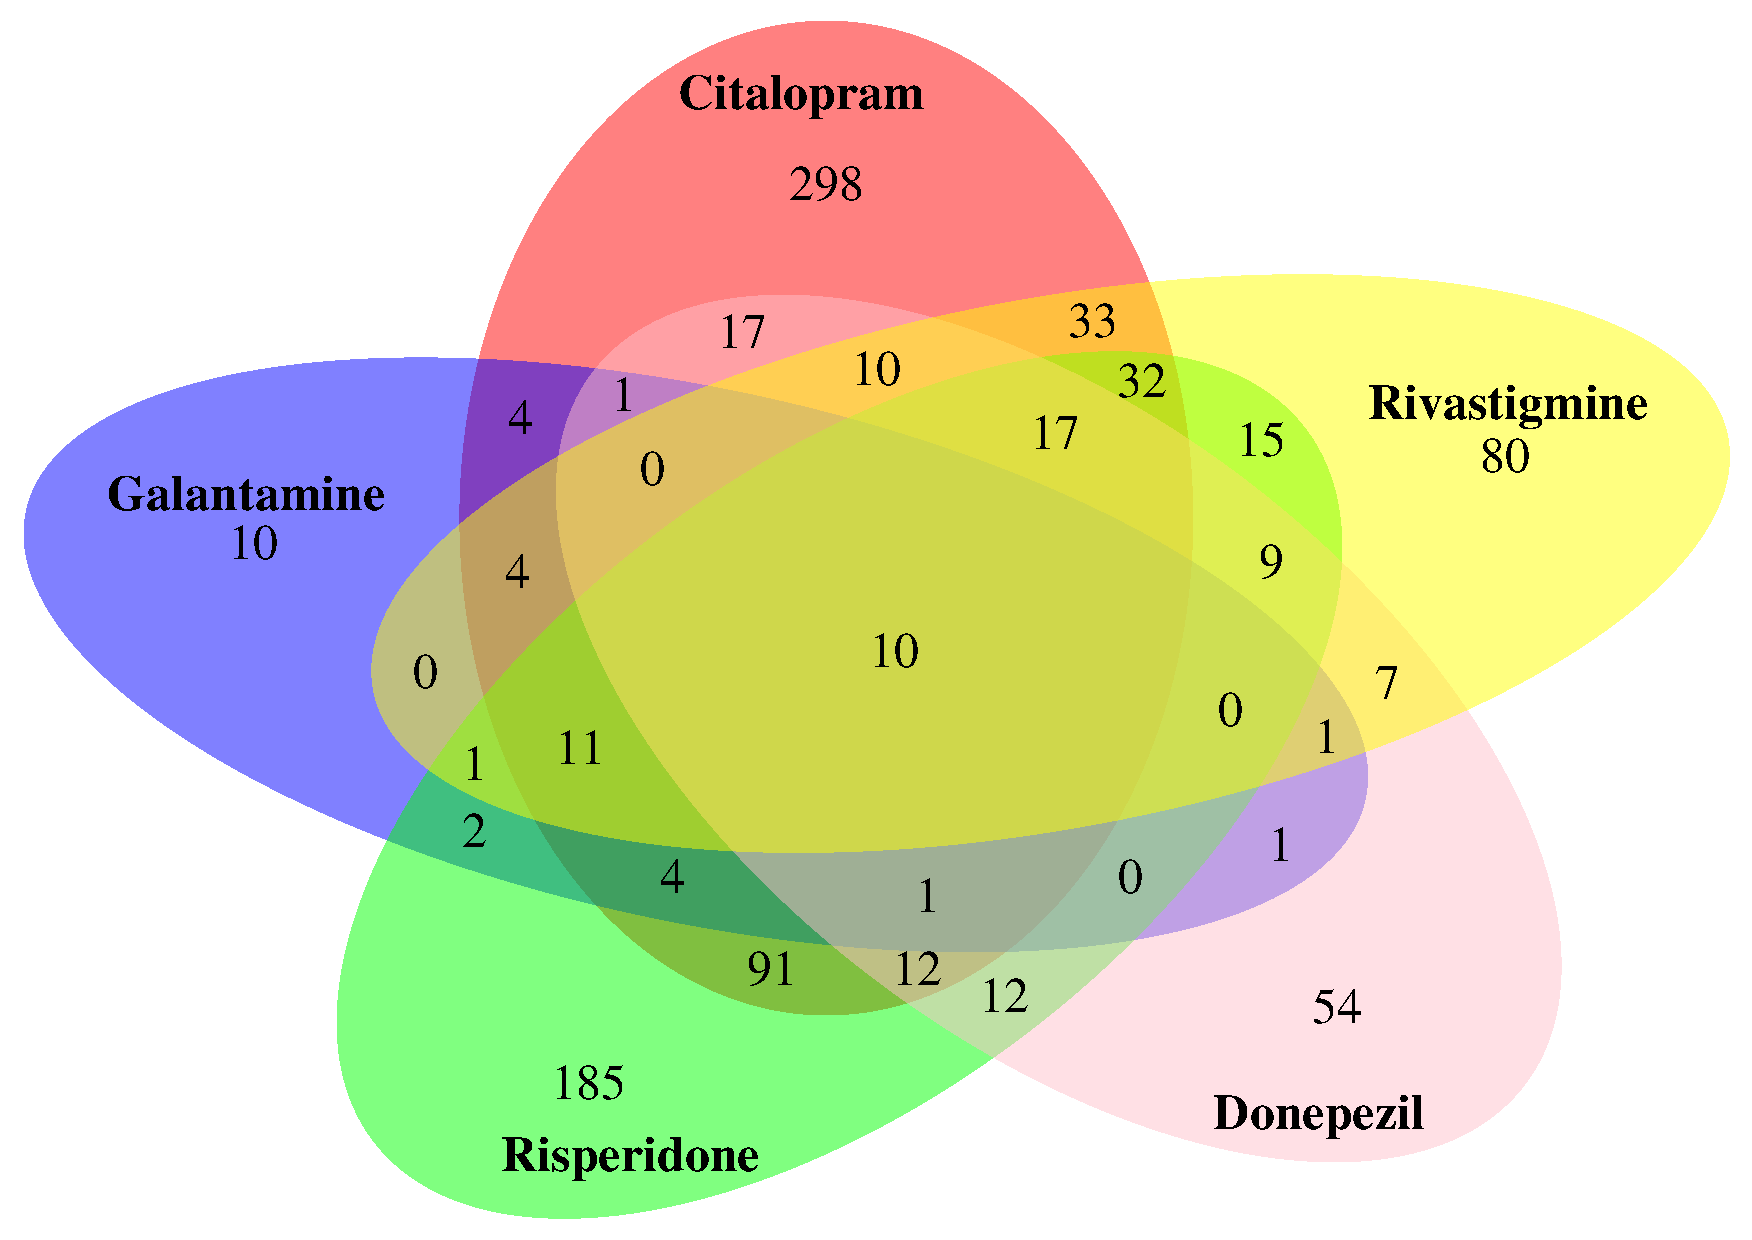
\includegraphics[width=9cm,height=8cm]{/LaTex/Reposition/venn-5.pdf} % OK
  \end{center}
\special{center} \caption{Venn diagram showing side-effects (shared and unique) between five of the nine main Alzheimer's drugs. 10 side-effects are common to all five drugs, using nine drugs we obtain eight side-effects.}
\label{venn}
\end{figure}
%%%%%%%%%%%%%%%%%%%%%%%%%%%

We decided to use the overlaps between the nine drugs as this allowed for 8 side-effects to be available for study, this simple approach proved to be quite powerful.  Initial work on the side-effects and known-targets can be found in \cite{McGarry2015a,McGarry2015b,McGarry2016a}. 

% latex table generated in R 3.3.2 by xtable 1.8-2 package
% Mon May 22 12:09:11 2017
\begin{table}[ht]
\centering \scriptsize \caption{List of shared side-effects common to all nine drugs}
\begin{tabular}{rl}
  \hline
 & side-effect \\ 
  \hline
1 & Apathy \\ 
  2 & Aphasia \\ 
  3 & Flat affect \\ 
  4 & Hypokinesia \\ 
  5 & Libido increased \\ 
  6 & Muscle contractions involuntary \\ 
  7 & Paranoia \\ 
  8 & Transient ischaemic attack \\ 
   \hline \normalsize
\end{tabular}
\label{se8}
\end{table}

The side-effects are typically what would be expected of drugs targeting the central nervous system. The drugs are used to either to slow the progress of dementia or to alleviate the worst symptoms of depression and anger. Algorithm 1, produced the following list of drugs shown in table \ref{drugs2repos}, we have displayed the top 25 drugs based on side-effect similarity of greater than 50\%. According to the Anatomical Therapeutic Chemical (ATC) codes, the majority of the drugs are `N', that is to say they are intended to target problems relating to the Nervous system. 

% latex table generated in R 3.3.2 by xtable 1.8-2 package
% Mon May 22 12:13:15 2017
\begin{table}[h]
\centering \scriptsize  \caption{Drugs with $>$ 50\% similarity. Where * may actually cause/exacerbate dementia related problems in some cases.}
\begin{tabular}{rlrrlll}
  \hline
 & Drugname & NoSideEffects & Similarity(\%) & drugbankid & atc\_codes&Repositioned? \\ 
  \hline
1 & Ropinirole & 418.00 & 100.00 & DB00268 & N04BC04 & Y\\ 
  2 & Bupropion & 288.00 & 87.50 & DB01156 & N06AX12 & Y\\ 
  3 & Pramipexole & 398.00 & 87.50 & DB00413 & N04BC05 & Y\\ 
  4 & Quetiapine & 188.00 & 87.50 & DB01224 & N05AH04 & Y\\ 
  5 & Selegiline & 216.00 & 87.50 & DB01037 & N04BD01 &Y\\ 
  6 & Sertraline & 208.00 & 87.50 & DB01104 & N06AB06 &Y\\ 
  7 & Topiramate & 301.00 & 87.50 & DB00273 & N03AX11&Y \\ 
  8 & Venlafaxine & 338.00 & 87.50 & DB00285 & N06AX16&Y \\ 
  9 & Gabapentin & 272.00 & 75.00 & DB00996 & N03AX12&Y \\ 
  10 & Lamotrigine & 152.00 & 75.00 & DB00555 & N03AX09&Y \\ 
  11 & Mirtazapine & 153.00 & 75.00 & DB00370 & N06AX11&Y* \\ 
  12 & Oxcarbazepine & 123.00 & 75.00 & DB00776 & N03AF02 &Y\\ 
  13 & Pregabalin & 561.00 & 75.00 & DB00230 & N03AX16 &N*\\ 
  14 & Cevimeline & 241.00 & 62.50 & DB00185 & N07AX03&N \\ 
  15 & Clomipramine & 221.00 & 62.50 & DB01242 & N06AA04&Y \\ 
  16 & Fluvoxamine & 221.00 & 62.50 & DB00176 & N06AB08&Y\\ 
  17 & Mycophenolate& 262.00 & 62.50 & DB00688 & L04AA06&N \\ 
  18 & Paroxetine & 362.00 & 62.50 & DB00715 & N06AB05 &N*\\ 
  19 & Pergolide & 156.00 & 62.50 & DB01186 & N04BC02& N\\ 
  20 & Rasagiline & 131.00 & 62.50 & DB01367 & N04BD02 &Y\\ 
  21 & Riluzole & 196.00 & 62.50 & DB00740 & N07XX02 &Y\\ 
  22 & Tiagabine & 102.00 & 62.50 & DB00906 & N03AG06&N \\ 
  23 & Tolcapone & 101.00 & 62.50 & DB00323 & N04BX01 &N\\ 
  24 & Tramadol & 373.00 & 62.50 & DB00193 & N02AX02 &N\\ 
  25 & Zolpidem & 129.00 & 62.50 & DB00425 & N05CF02 &Y*\\  
   \hline
\end{tabular} \normalsize
\label{drugs2repos}
\end{table}

Some of the drugs have been used to treat the symptoms of Alzheimer's disease such as depression, anxiety etc. Some have actually been used with a view to halt the degenerative process. Table \ref{drugs1}  provides a few more details of the characteristics for the first five drugs and any applications for Alzheimer's disease. 


\scriptsize
\begin{table}[h!]
\scriptsize
  \centering \caption{Details of drugs 1-5 }\label{drugs1}
  \begin{tabular}{ | c | m{4.5cm} | m{4.5cm} | }
    \hline
    Drug structure & Original use & Repositioned for Alzheimer's? \\ \hline
    \begin{minipage}{.3\textwidth}
      \includegraphics[width=\linewidth, height=2cm]{/LaTex/Reposition/ropinrole.jpg}
    \end{minipage}
    & ROPINIROLE
    %\begin{minipage}[t]{5cm}
      \begin{itemize}
         \item A dopamine agonist. Commonly used to treat restless legs and Parkinson syndrome. It works by increasing the level of dopamine in the brain.
        \item Research  supports that the influx of dopamine does improve the blood flow in the brain. Possible candidate.
      \end{itemize}
    %\end{minipage}
    & 
    %\begin{minipage}{5cm}
      \begin{itemize}
        \item Improved Alzheimer’s related depression.
      \end{itemize}
    %\end{minipage}
    \\ \hline
    %=============================================
     \begin{minipage}{.3\textwidth}
      \includegraphics[width=\linewidth, height=2cm]{/LaTex/Reposition/Bupropion_1.jpg}
    \end{minipage}
    & BUPROPION
    %\begin{minipage}[t]{5cm}
      \begin{itemize}
        \item Bupropion is an antidepressant medication used to treat major depressive disorder and seasonal affective disorder.
         
      \end{itemize}
    %\end{minipage}
    & 
    %\begin{minipage}{5cm}
      \begin{itemize}
        \item Reduced apathy in Alzheimer's patients 
        \item Incipient Alzheimer's disease is often disguised as depressive disorder.
            \end{itemize}
    %\end{minipage}
    \\ \hline
    
    %=============================================
     \begin{minipage}{.3\textwidth}
      \includegraphics[width=\linewidth, height=2cm]{/LaTex/Reposition/pramip.jpg}
    \end{minipage}
    & PRAMIPEXOLE
    %\begin{minipage}[t]{5cm}
      \begin{itemize}
        \item Pramipexole is a selective dopamine receptor agonist used in the therapy of Parkinson disease. 
         
      \end{itemize}
    %\end{minipage}
    & 
    %\begin{minipage}{5cm}
      \begin{itemize}
        \item counteract the problems with low libido experienced by some users of SSRI antidepressant drugs. Pramipexole has shown robust effects on pilot studies in bipolar disorder.
            \end{itemize}
    %\end{minipage}
    \\ \hline
        %=============================================
     \begin{minipage}{.3\textwidth}
      \includegraphics[width=\linewidth, height=2cm]{/LaTex/Reposition/quit.jpg}
    \end{minipage}
    & QUETIAPINE
    %\begin{minipage}[t]{5cm}
      \begin{itemize}
        \item Used treatment of Parkinson's, schizophrenia, bipolar disorder, and major depressive disorder. It is also sometimes used as a sleep aid due to its sedating effect. 
       
      \end{itemize}
    %\end{minipage}
    & 
    %\begin{minipage}{5cm}
      \begin{itemize}
        \item Used to treat for hallucinations, delusions, aggression, agitation in Alzheimer patents.
            \end{itemize}
    %\end{minipage}
    \\ \hline
    %=============================================
     \begin{minipage}{.3\textwidth}
      \includegraphics[width=\linewidth, height=2cm]{/LaTex/Reposition/seg.jpg}
    \end{minipage}
    & SEGEGILINE
    %\begin{minipage}[t]{5cm}
      \begin{itemize}
        \item Selegiline  is used to treat movement disorders caused by Parkinson's disease. Not a cure for Parkinson's disease, but it may improve tremor.

      \end{itemize}
    %\end{minipage}
    & 
    %\begin{minipage}{5cm}
      \begin{itemize}
        \item Selegiline treatment for symptoms of Alzheimer's disease remains controversial and is reflected by its low rate of prescription and the lack of approval by several regulatory authorities in Europe and elsewhere. 
            \end{itemize}
    %\end{minipage}
    \\ \hline
  \end{tabular}
 \end{table}
\normalsize

The candidate drugs at the lower end of our similarity scale such as Tramadol, an analgesic drug, affects the peripheral and central nervous system \cite{Minami2015}. Tramadol, an opioid is mainly used to treat pain,  in terms of Alzheimer's, patients are advised to avoid it, as it appears to worsen the condition.  This is as it has anti-cholinergic side effects. It causes serious side effects like serotonin syndrome, this is due to the influx of the neurotransmitter serotonin and then it inhibits the reuptake of serotonin, which can cause toxic levels. This could be a possible reason for tramadol worsening the condition of Alzheimer sufferers. Side effects like confusion and agitation worsen for Alzheimer patients on tramadol, the effects seem to be severe in the elderly \cite{Vazzana2015}.

Zolpidem actually appears to be implicated with causing dementia when underlying diseases, such as hypertension and diabetes after controlling for potential confounders, such as age, sex, coronary artery disease, diabetes and anti-hypertension drugs are taken into account.


In table \ref{candidatetreats} for 10 of our candidate drugs we have presented for each drug up to five of the original diseases and symptoms they were designed to treat. On average each drug was used to treat 21 diseases/indications, the minimum was one disease and the maximum value was 88 diseases.

\begin{table}[h]
\scriptsize
  \centering \caption{Top 10 candidate drugs and the problems/symptoms they were designed to treat}\label{candidatetreats}
\centering
\begin{tabular}{ll}
  \hline
  Drug & Disease/indications \\ \hline
Ropinirole  & Hypotension, Muscle rigidity, Parkinson's disease, Restless legs syndrome, Tachycardia    \\
Bupropion  & Mental disorder, Depression, Dysthymic disorder, Fatigue, Asthenia\\        
Pramipexole & Parkinsonism, Parkinson's disease, Restless legs syndrome\\
Quetiapine & Mental disorder, Bipolar disorder, Bipolar I disorder,  Psychotic disorder, Depression\\
Selegiline   & Fatigue, Asthenia, Feeling guilty, Major depression, Parkinson's disease\\
Sertraline   & Agoraphobia, Anger, Anxiety, Depression, Dysthymic disorder\\    
Topiramate & Bipolar disorder, Cluster headache, Migraine, Epilepsy, Partial seizures\\
Venlafaxine & Agoraphobia, Anxiety, Chest pain, Depersonalisation, Depression   \\ 
Gabapentin & Ataxia, Diabetes mellitus, Dizziness, Epilepsy, Erythema multiforme, Fatigue  \\
Lamotrigine & Bipolar disorder, Dysmenorrhoea, Epilepsy, Grand mal convulsion, Parkinson's disease  \\
   \hline \normalsize
\end{tabular}
\end{table}

\subsection{Analysis of the chemical structures and protein targets}
A computational model was built using the chemical data from drugbank, this indicates the connectivity patterns linking drug to target receptors. We downloaded the relevant structure data files (SDF) for the 77 drugs (69 candidate drugs and 8 current drugs) using their drugbank identifiers, The atom-pairs are converted into molecular fingerprints and these are clustered. 

We created a chemical fingerprint for each of the drugs, we chose 2048 atom-pairs although it is possible to use a structure containing 4096 most common atom pairs in DrugBank. The pairwise distances are calculated for all 77 entries (69 candidate drugs and 8 current drugs) between the given fingerprints and then fit a Beta distribution to the resulting Tanimoto scores, conditioned on the number of set bits in each fingerprint. In table \ref{comp1} we show the chemical similarity for 25 candidate drugs with the three main Alzheimer's drugs, individually and overall.


\begin{table}[h]
\scriptsize
  \centering \caption{Chemical similarity measures for the candidate drugs based on 2048-length fingerprints compared with the three most common treatments for slowing disease progression, only first 25 are shown}\label{comp1}
\centering
\begin{tabular}{llllll}
  \hline
 & name & similarity & similarity & similarity & overall score\\ 
              &                   & (Rivastigmine) & (Galantamine)  & (Donepezil)          & \\
  \hline 
  
% 1 & Galantamine & 0.20 & 1.00 & 0.26 & 0.49 \\ 
% 2 & Donepezil & 0.15 & 0.26 & 1.00 & 0.47 \\ 
%  3 & Rivastigmine & 1.00 & 0.20 & 0.15 & 0.45 \\ 
  1 & Pergolide & 0.21 & 0.46 & 0.39 & 0.35 \\ 
  2 & Tramadol & 0.42 & 0.27 & 0.27 & 0.32 \\ 
  3 & Haloperidol & 0.13 & 0.16 & 0.65 & 0.31 \\ 
  4 & Citalopram & 0.23 & 0.36 & 0.30 & 0.30 \\ 
  5 & Escitalopram & 0.23 & 0.36 & 0.30 & 0.30 \\ 
  6 & Clomipramine & 0.24 & 0.33 & 0.32 & 0.29 \\ 
  7 & Hydromorphone & 0.15 & 0.42 & 0.30 & 0.29 \\ 
  8 & Tiagabine & 0.12 & 0.36 & 0.39 & 0.29 \\ 
  9 & Sibutramine & 0.28 & 0.33 & 0.25 & 0.29 \\ 
  10 & Mirtazapine & 0.20 & 0.39 & 0.28 & 0.29 \\ 
  11 & Bupropion & 0.50 & 0.21 & 0.16 & 0.29 \\ 
  12 & Venlafaxine & 0.26 & 0.27 & 0.32 & 0.28 \\ 
  13 & Morphine & 0.16 & 0.50 & 0.18 & 0.28 \\ 
  14 & Trazodone & 0.16 & 0.17 & 0.51 & 0.28 \\ 
  15 & Zolmitriptan & 0.27 & 0.31 & 0.25 & 0.28 \\ 
  16 & Ropinirole & 0.15 & 0.32 & 0.35 & 0.27 \\ 
  17 & Zuclopenthixol & 0.13 & 0.26 & 0.42 & 0.27 \\ 
  18 & Quetiapine & 0.12 & 0.27 & 0.42 & 0.27 \\ 
  19 & Sumatriptan & 0.27 & 0.32 & 0.21 & 0.27 \\ 
  20 & Sertraline & 0.26 & 0.30 & 0.23 & 0.27 \\ 
  21 & Doxazosin & 0.13 & 0.23 & 0.44 & 0.27 \\ 
  22 & Riluzole & 0.39 & 0.22 & 0.16 & 0.26 \\ 
  23 & Rasagiline & 0.32 & 0.27 & 0.18 & 0.26 \\ 
  23 & Nicotine & 0.41 & 0.19 & 0.16 & 0.25 \\ 
  25 & Varenicline & 0.19 & 0.33 & 0.23 & 0.25 \\ 
   \hline
\end{tabular}
\end{table}

In table \ref{comp1}  the highest matching drug is similarity is  Pergolide with a 35\% commonality. The majority of drugs have between 32\% and 25\% chemical similarity. Since these all these candidate drugs had similar side-effects and since their chemical composition is quite different, we can conclude that chemical similarity alone should not be used to seek out drugs for re-purposing.

Using hierarchical clustering on the drug similarity matrix provides a little bit more information. Through a process trial and error we deduced that there are 10 clusters. The validity of clusters in terms of composition is more or less confirmed by the similarity matrix. However, analysis of the chemical similarity matrix does not provide a full explanation and further integration of data is needed. 

The silhouette plot in figure \ref{fig:sillo} indicates that the majority of the drug clusters are reasonably good in terms of quality of fit. Values near one (unity) indicates  that the observation is well placed in its cluster; values near zero show that it's likely that an observation should belong to some other cluster. 

\begin{itemize}
\item 0.71-1.0  - A strong structure has been found
\item 0.51-0.70 - A reasonable structure has been found
\item 0.26-0.50 - The structure is weak and could be artificial
\item $<$ 0.25 No substantial structure has been found
\end{itemize}


\begin{figure}[h]
  \begin{subfigure}[b]{0.3\textwidth}
    \includegraphics[angle=270,width=8cm,totalheight=10cm]{/LaTex/Reposition/dendro2.pdf} % OK
    \caption{Dendrogram of clusters}
    \label{fig:dendro}
  \end{subfigure}
  \hfill
  \begin{subfigure}[b]{0.5\textwidth}
    \includegraphics[width=8cm,height=10cm]{/LaTex/Reposition/silhouette.pdf} % O
    \caption{Silhouette plot determining goodness of fit of the clusters.}
    \label{fig:sillo}
  \end{subfigure}
  \caption{Clustering the 69 candidate drugs and eight conventional treatment drugs, 10 clusters are identified based on the chemical similarity matrix. The silhouette plot indicates goodness of fit}
\end{figure}


We can therefore conclude that chemical similarity is no guarantee that a drug will have the similar therapeutic qualities or be beneficial somehow. The chemical information must be collated with higher level biological knowledge and known protein interactions for a deeper and more accurate indication of the usefulness of the candidate drugs.  


\subsection{Disease similarity analysis using the disease ontology}
For each of the 69 candidate drugs we note the disease/symptoms each one is targeted against and produce a correlation  matrix from the terms annotating each disease from the disease ontology. Observing the correlation values (using Wang similarity measure) we can see the terms are reasonably similar between Parkinson's and Alzheimer's disease. In figure \ref{dose1} the main types of diseases treated by the 13 drugs are shown. The similarity measure is constrained to lie between 0 and 1, with 1 being the highest level of similarity. Ignoring the diagonal, the highest measure is between psychosis and schizophrenia (0.64) and between Parkinson's and Alzheimer's (0.44), depression and psychosis (0.39), followed by epilepsy and Alzheimer's (0.35). Description of correlational strength is based on Cohen's measures where very high 0.9 - 1.0; high 0.7 - 0.9; moderate 0.5 - 0.7 ; low 0.3 - 0.5.


%%%%%%% Figure %%%%%%%%%%%%%%%%
\begin{figure}[h]
%\epsfysize=4.0cm \leavevmode
  \begin{center}
	 \includegraphics[width=11cm,height=9cm]{/LaTex/Reposition/DOSE.pdf} % OK
  \end{center}
\special{center} \caption{Disease ontology similarity matrix, the correlations are based `off the diagonal' and take on values between 0 and 1.}
\label{dose1}
\end{figure}
%%%%%%%%%%%%%%%%%%%%%%%%%%%

Overall, we find 48 terms used to describe the diseases  in a hierarchy. Through extensive cross-mapping of DO terms to standard clinical and medical terminologies of MeSH, ICD, NCI's thesaurus, SNOMED and OMIM it can reflect the current knowledge of human diseases and their associations with phenotype, environment and genetics.  In table \ref{doterms} the 48 terms assigned to the 10 diseases are shown, in addition to exact matches the Wang measure also assesses the semantic similarity.


% latex table generated in R 3.2.2 by xtable 1.8-2 package
% Fri Jul 29 09:07:48 2016
\begin{table}[h]
\centering \scriptsize \caption{48 DO terms assigned to the diseases}\label{doterms}
\begin{tabular}{rlrl}
  \hline
 & &  \\ 
  \hline
1 & degenerative disease & 25 & syndrome \\ 
  2 & rheumatism & 26  &disease \\ 
  3 & psychotic disorder & 27 &delirium, dementia, cognitive disorder \\ 
  4 & Movement disorder & 28&cerebral degeneration \\ 
  5 & organic brain syndrome & 29&organic psychosis \\ 
  6 & central nervous system disease & 30& Tauopathies \\ 
  7 & neurodegenerative disorder & 31&dementia \\ 
  8 & Parkinsonian disorder & 32&endogenous depression \\ 
  9 & body system disease & 33&episodic mood disorder \\ 
  10 & musculoskeletal system disease & 34&mental depression \\ 
  11 & nervous system disease &35& Autonomic nervous system disorder \\ 
  12 & peripheral nervous system disease & 36&peptic ulcer \\ 
  13 & hereditary degenerative disease of central nervous system & 37&gastrointestinal system disease \\ 
  14 & neuromuscular disease & 38&disease by infectious agent \\ 
  15 & neuropathy & 39&opportunistic mycosis \\ 
  16 & disease of biological process & 40&lentivirus infectious disease \\ 
  17 & disease of behavior & 41&viral infectious disease \\ 
  18 & disease of anatomical entity & 42&AIDS-related opportunistic infectious disease \\ 
  19 & Muscle, ligament and fascia disorder & 43&RNA virus infectious disease \\ 
  20 & myopathy & 44&HIV infectious disease \\ 
  21 & soft tissue disease & 45&retroviridae infectious disease \\ 
  22 & tissue disease & 46&fungal infectious disease \\ 
  23 & brain disease & 47&reproductive system disease \\ 
  24 & basal ganglia disease & 48&female reproductive system disorder \\ 
   \hline
\end{tabular}
\end{table}
\normalsize

\subsection{Enrichment analysis of proteins using gene ontology}
The protein networks can be further enhanced by integrating known biological knowledge from gene ontology \cite{Ashburner00, Deng04}. This information illuminates biological pathways, signaling mechanisms, genes, associated diseases that the proteins are involved in and indicates where the drug of interest is active.  The information is important since the drug will often interact with off-targets, identifying these interactions will often lead to an explanation of why a drug has particular side-effects. In figure \ref{pathway1} the biological pathways involved with all of our target proteins are displayed.

%%%%%%% Figure %%%%%%%%%%%%%%%%
\begin{figure}[h]
%\epsfysize=4.0cm \leavevmode
  \begin{center}
	 \includegraphics[width=14cm,height=11cm]{/LaTex/Reposition/ontargetpaths1.pdf} % OK
	 %\includegraphics[trim={722 74 1091 1091},clip]{/LaTex/Reposition/enrich1.eps} %
	% trim={<left> <lower> <right> <upper>}
   \end{center}
\special{center} \caption{Biological pathway involvement attributed to the on-target proteins associated with all candidate drugs}
\label{pathway1}
\end{figure}
%%%%%%%%%%%%%%%%%%%%%%%%%%%

The pathways presented in figure \ref{pathway1} play a role in a number of important cellular and metabolic processes, when this pathway annotation is integrated with the other drug-to-protein networks we are able to discern a number of overlapping functions and processes. Observing the enrichment process we can see that proteins implicated with the same disease (and related diseases) are more predisposed to interact with each other rather than interact with other proteins. These proteins also have common GO terms and are likely to be located in the same tissues. Proximity, in protein-protein networks as borne out by the network statistics is an important factor. Disease genes appear to high degree but low clustering coefficients.

% latex table generated in R 3.3.2 by xtable 1.8-2 package
% Thu Jun 01 11:55:32 2017
\begin{table}[h]
\centering \scriptsize \caption{Example of GO Biological Process terms related to the on-target proteins for all candidate drugs}\label{goterms}
\begin{tabular}{rllllr}
  \hline 
 & ID & Description & GeneRatio & BgRatio & pvalue  \\ 
  \hline
1 & 375280 & Amine ligand-binding receptors & 30/156 & 36/6748 & 0.00 \\ 
  2 & 211981 & Xenobiotics & 15/156 & 17/6748 & 0.00 \\ 
  3 & 112315 & Transmission across Chemical Synapses & 36/156 & 194/6748 & 0.00  \\ 
  4 & 112316 & Neuronal System & 39/156 & 274/6748 & 0.00 \\ 
  5 & 211945 & Phase 1 - Functionalization of compounds & 23/156 & 73/6748 & 0.00 \\ 
  6 & 211859 & Biological oxidations & 29/156 & 149/6748 & 0.00 \\ 
  7 & 211897 & Cytochrome P450 - arranged by substrate type & 19/156 & 55/6748 & 0.00  \\ 
  8 & 112314 & Neurotransmitter Receptor Binding  & 26/156 & 137/6748 & 0.00 \\ 
  9 & 373076 & Class A/1 (Rhodopsin-like receptors) & 36/156 & 307/6748 & 0.00 \\ 
  10 & 975298 & Ligand-gated ion channel transport & 13/156 & 25/6748 & 0.00 \\ 
  11 & 390666 & Serotonin receptors & 10/156 & 12/6748 & 0.00 \\ 
  12 & 629594 & Highly calcium permeable postsynaptic nicotinic acetylcholine receptors & 10/156 & 12/6748 & 0.00 \\ 
  13 & 500792 & GPCR ligand binding & 38/156 & 392/6748 & 0.00 \\ 
  14 & 181431 & Acetylcholine Binding And Downstream Events & 10/156 & 15/6748 & 0.00 \\ 
  15 & 622327 & Postsynaptic nicotinic acetylcholine receptors & 10/156 & 15/6748 & 0.00 \\ 
   \hline \normalsize
\end{tabular}
\end{table}

\subsection{Complex network analysis of protein connectivity patterns and biological pathways}
Protein interaction connectivity patterns represent important biological functions and signaling mechanisms.  The drugs designed to combat diseases are targeted at specific proteins but unfortunately also affect off-targets and create side-effects. Furthermore, proteins tend to operate together in modules that perform specific functions and that proteins can belong to several modules. It is therefore essential to build up a complete profile of the drugs and their interaction partners. 

Diagrams are of limited use when displaying connectivity patterns of complex networks, even the small networks can easily become incomprehensible  and visually are of limited use. The network statistics based on the values of hubness, closeness and betweeness provide a deeper understanding of the connectivity patterns than a visual assessment. The protein targets and known protein interactions of the 25 drugs were identified, downloaded from the relevant database (STITCH) and complex network analysis was applied to the subsequent network structures.  We created 25 separate protein-to-drug interaction networks and calculated the relevant statistics for each and then combined the 25 networks into one large interaction network and recalculated the statistics. 

The statistics for the 25 drug networks is shown in table \ref{twentyfive}, every network has individual values for each protein (not shown) in terms of hubness and betweenness. The number of edges, number nodes, the modularity, and average path will be identical for each protein in a given network. It should be stated that these networks are both off and on-targets and the data is from STITCH.


\begin{table}[h]
\centering \caption{Complex network statistics for the 25 candidate drug networks (individually) } \label{twentyfive}
\scriptsize
\begin{tabular}{lllllllllll}
\hline
   drug & modularity & avepath & nedges & nverts & transit & degree & clos & between & dens & hubness \\ 
  \hline
 bupropion & 0.245 & 2 & 72 &   23 & 1 & 2.000 & 0.022 & 0.000 & 0.285 & 0.126 \\ 
  cevimeline & 0.086 & 2 & 46 &   15 & 1 & 6.000 & 0.045 & 27.179 & 0.438 & 0.511 \\ 
  citalopram & 0.286 & 2 & 209 &   44 & 0 & 43.000 & 0.023 & 565.914 & 0.221 & 1.000 \\ 
  clomipramine & 0.396 & 2 & 183 &   49 & 0 & 48.000 & 0.021 & 879.129 & 0.156 & 1.000 \\ 
  fluvoxamine & 0.363 & 2 & 81 &   39 & 0 & 38.000 & 0.026 & 622.633 & 0.109 & 1.000 \\ 
  gabapentin & 0.367 & 2 & 78 &   32 & 0 & 31.000 & 0.032 & 387.317 & 0.157 & 1.000 \\ 
  lamotrigine & 0.427 & 2 & 127 &   40 & 0 & 39.000 & 0.026 & 590.368 & 0.163 & 1.000 \\ 
  mirtazapine & 0.442 & 2 & 214 &   51 & 1 & 50.000 & 0.020 & 943.046 & 0.168 & 1.000 \\ 
  mycophenolic & 0.424 & 2 & 88 &   30 & 0 & 29.000 & 0.034 & 325.793 & 0.202 & 1.000 \\ 
  oxcarbazepine & 0.221 & 2 & 24 &   14 & 0 & 13.000 & 0.077 & 61.500 & 0.264 & 1.000 \\ 
  paroxetine & 0.319 & 2 & 127 &   33 & 0 & 32.000 & 0.031 & 301.926 & 0.241 & 1.000 \\ 
  pergolide & 0.358 & 2 & 123 &   33 & 1 & 32.000 & 0.031 & 352.400 & 0.233 & 1.000 \\ 
  pregabalin & 0.030 & 2 & 13 &    8 & 1 & 7.000 & 0.143 & 13.333 & 0.464 & 1.000 \\ 
  abanoquil & 0.055 & 1 & 131 &   21 & 1 & 2.000 & 0.023 & 0.000 & 0.624 & 0.109 \\ 
  rasagiline & 0.114 & 2 & 33 &   12 & 1 & 11.000 & 0.091 & 17.817 & 0.500 & 1.000 \\ 
  riluzole & 0.333 & 2 & 72 &   31 & 0 & 30.000 & 0.033 & 357.500 & 0.155 & 1.000 \\ 
  ropinirole & 0.361 & 2 & 77 &   25 & 1 & 24.000 & 0.042 & 209.833 & 0.257 & 1.000 \\ 
  selegiline & 0.220 & 2 & 152 &   36 & 0 & 26.000 & 0.023 & 190.501 & 0.241 & 1.000 \\ 
  sertraline & 0.356 & 2 & 153 &   49 & 0 & 48.000 & 0.021 & 912.696 & 0.130 & 1.000 \\ 
  tiagabine & 0.166 & 2 & 13 &   11 & 0 & 10.000 & 0.100 & 40.500 & 0.236 & 1.000 \\ 
  tolcapone & 0.079 & 2 & 14 &    9 & 0 & 8.000 & 0.125 & 19.000 & 0.389 & 1.000 \\ 
  topiramate & 0.367 & 2 & 68 &   34 & 0 & 33.000 & 0.030 & 472.843 & 0.121 & 1.000 \\ 
  tramadol & 0.257 & 2 & 21 &   14 & 0 & 13.000 & 0.077 & 68.000 & 0.231 & 1.000 \\ 
  venlafaxine & 0.230 & 2 & 82 &   39 & 0 & 38.000 & 0.026 & 627.945 & 0.111 & 1.000 \\ 
  zolpidem & 0.035 & 1 & 160 &   24 & 1 & 23.000 & 0.043 & 116.000 & 0.580 & 1.000 \\ 
   \hline
\end{tabular}
\end{table}
 \normalsize


%%%%%%%%%%%% COMMENTED OUT FOR THE MOMENT %%%%%%%%%%%%%%%%
\begin{comment}
The statistics shown in table \ref{giant1} refers to the combined network of the 13 smaller networks, the values for each drug in terms of  degree, number of edges, number of vertices, betweeness and hubness will be different to their individual networks since many proteins are shared once they are combined into the larger network. Creating the large drug network is essential to understand the various protein interactions as a whole, rather than viewing them as isolated drugs.
% latex table generated in R 3.2.2 by xtable 1.8-2 package
% Tue Jul 19 12:31:28 2016
\begin{table}[h]
\centering \caption{Complex network statistics for the drugs in the large combined network of 973 edges and 169 nodes. The table is ordered according to the hubness statistic. The large network has a modularity of 0.419, average path of 2.72 and transitivity of 0.40}\label{giant1}
\scriptsize
\begin{tabular}{llll}
  \hline
 & degree & betweeness & hubness \\ 
  \hline
  olanzapine & 50 & 1088.456 & 0.923 \\ 
  aripiprazole & 40 & 648.749 & 0.766 \\ 
  fluoxetine & 50 & 2866.827 & 0.755 \\ 
  citalopram & 43 & 1458.980 & 0.652 \\ 
  paroxetine & 32 & 1077.320 & 0.503 \\ 
  ropinirole & 24 & 603.617 & 0.446 \\ 
  tramadol & 13 & 487.397 & 0.176 \\ 
  donepezil & 16 & 561.330 & 0.139 \\ 
  naltrexone & 13 & 607.161 & 0.105 \\ 
  ofloxacin & 21 & 1161.053 & 0.093 \\ 
  rivastigmine & 5 & 169.852 & 0.059 \\ 
  galantamine & 4 & 2.852 & 0.059 \\ 
  pregabalin & 7 & 415.833 & 0.002 \\ 
   \hline
\end{tabular}
\end{table}
\normalsize
\end{comment}
%%%%%%%%%%%%%%%%%%%%%%%%%%%%%%%%%%%%%

Although drugs act at the level of protein/enzyme interactions, their overall effect is to modify the cells processes or signaling mechanisms that comprise important biological pathways. A biological pathway can be described as a collection of ordered, discrete actions among molecules that can breakdown proteins or assemble them in the cell. Such a pathway can trigger the assembly of new molecules by turning genes on and off. There are several types of pathways that control metabolism, signaling cascades, transport and otherwise generally control the behavior and actions of the cell in response to stimuli. The normal healthy body requires the coordination of many biological pathways, the majority of diseases involve the malfunction of proteins that cooperate in pathways. In fact 30\% of drugs operate on one type of protein called G protein-coupled receptors (GPCRS). 

%%%%%%% Figure %%%%%%%%%%%%%%%%
\begin{figure}[h]
%\epsfysize=4.0cm \leavevmode
  \begin{center}
	\centering \includegraphics[width=8cm,height=8cm]{/LaTex/Reposition/roc.pdf} % OK
  \end{center}
\centering \caption{ROC curves for the goodness of fit of the complex latent network model. The green curve represents the combined protein-interactions+ontology+pathways. Blue curve is the protein-interactions + pathways, Red curve is the protein-interactions alone}
\label{roc}
\end{figure}
%%%%%%%%%%%%%%%%%%%%%%%%%%%

In addition to the complex network statistics of drug to protein interactions, we also evaluated the drugs intended on-target protein interactions and their relationships using latent variables. This data was obtained from drugbank and contains different information to STITCH. We are interested in variables that are unobserved but play a role in determining the probability that vertex pairs (drug to protein and protein to protein) are incident to each other \cite{Kolaczyk2014} . In figure \ref{roc} we plot the ROC curves for the latent network. We use eigenmodels with 5-fold cross-validation using MCMC to simulate the posterior distributions. We take the typical values of 10,000 for burn-in and 1,000 for inferencing. This allows us to model the effects of using: 1. protein and drug interactions alone, 2. protein interactions + pathways, 3. protein interactions + pathways + level  2 ontology. The AUC's for the three models are 73\%, 86\% and 90\% respectively. Increasing the amount of information provides the complex network with greater, internal robustness, 

\subsection{Data integration and drug scoring}
The sources of data are merged in a principled way using the drug integration scoring scheme described in equation \ref{integrate}.  Each source of data was integrated using the Jaccard measure. Based on  the linear equation the sources of data were each allocated a coefficient (similar to regression) and a matrix was produced for each drug. The diagonal contains the combined Jaccard score for each drug. This was used to reevaluate the initial list of candidate drugs as determined by side-effect similarity alone. Referring to table \ref{newlist}, the initial ranking (table \ref{drugs2repos}) determined by side-effect similarity alone has changed somewhat. Ropinirole is still the top scoring drug but the positions of the majority of the drugs has changed and the last three drugs were not on the original list of 25 having moved up the list.

\begin{table}[h]
\centering \scriptsize \caption{Final ranked list of candidate drugs for Alzheimer's disease}\label{newlist}
\begin{tabular}{rllllr}
  \hline
 & drugbank\_id & name & type & atc\_codes & overall score \\ 
  \hline
1 & DB00268 & Ropinirole & small molecule & N04BC04 & 0.81 \\ 
  2 & DB00413 & Pramipexole & small molecule & N04BC05 & 0.66 \\ 
  3 & DB00273 & Topiramate & small molecule & N03AX11 & 0.66 \\ 
  4 & DB01037 & Selegiline & small molecule & N04BD01 & 0.65 \\ 
  5 & DB01156 & Bupropion & small molecule & N06AX12 & 0.64 \\ 
  6 & DB00285 & Venlafaxine & small molecule & N06AX16 & 0.60 \\ 
  7 & DB01104 & Sertraline & small molecule & N06AB06 & 0.58 \\ 
  8 & DB01224 & Quetiapine & small molecule & N05AH04 & 0.57 \\ 
  9 & DB00230 & Pregabalin & small molecule & N03AX16 & 0.56 \\ 
  10 & DB00776 & Oxcarbazepine & small molecule & N03AF02 & 0.56 \\ 
  11 & DB00555 & Lamotrigine & small molecule & N03AX09 & 0.54 \\ 
  12 & DB00996 & Gabapentin & small molecule & N03AX12 & 0.52 \\ 
  13 & DB00370 & Mirtazapine & small molecule & N06AX11 & 0.45 \\ 
  14 & DB00323 & Tolcapone & small molecule & N04BX01 & 0.44 \\ 
  15 & DB01367 & Rasagiline & small molecule & N04BD02 & 0.43 \\ 
  16 & DB00906 & Tiagabine & small molecule & N03AG06 & 0.43 \\ 
  17 & DB00185 & Cevimeline & small molecule & N07AX03 & 0.42 \\ 
  18 & DB00740 & Riluzole & small molecule & N07XX02 & 0.42 \\ 
  19 & DB00425 & Zolpidem & small molecule & N05CF02 & 0.40 \\ 
  20 & DB00193 & Tramadol & small molecule & N02AX02 & 0.40 \\ 
  21 & DB01186 & Pergolide & small molecule & N04BC02 & 0.38 \\ 
  22 & DB01242 & Clomipramine & small molecule & N06AA04 & 0.37 \\ 
  23 & DB00688 & Mycophenolate mofetil & small molecule & L04AA06 & 0.37 \\ 
  24 & DB00176 & Fluvoxamine & small molecule & N06AB08 & 0.37 \\ 
  25 & DB00715 & Paroxetine & small molecule & N06AB05 & 0.33 \\ 
%  26 & DB00659 & Acamprosate & small molecule & N07BB03 & 0.32 \\ 
%  27 & DB00494 & Entacapone & small molecule & N04BX02 & 0.32 \\ 
 % 28 & DB01105 & Sibutramine & small molecule & A08AA10 & 0.31 \\ 
  %29 & DB00853 & Temozolomide & small molecule & L01AX03 & 0.31 \\ 
  %30 & DB00949 & Felbamate & small molecule & N03AX10 & 0.30 \\ 
  %31 & DB00625 & Efavirenz & small molecule & J05AG03 & 0.29 \\ 
  %32 & DB00327 & Hydromorphone & small molecule & N02AA03 & 0.28 \\ 
  %33 & DB01624 & Zuclopenthixol & small molecule & N05AF05 & 0.28 \\ 
  %34 & DB00915 & Amantadine & small molecule & N04BB01 & 0.28 \\ 
  %35 & DB00216 & Eletriptan & small molecule & N02CC06 & 0.28 \\ 
  %36 & DB00669 & Sumatriptan & small molecule & N02CC01 & 0.28 \\ 
  %37 & DB00448 & Lansoprazole & small molecule & A02BC03 & 0.27 \\ 
  %38 & DB00656 & Trazodone & small molecule & N06AX05 & 0.27 \\ 
  %39 & DB01149 & Nefazodone & small molecule & N06AX06 & 0.26 \\ 
  %40 & DB00537 & Ciprofloxacin & small molecule & S01AE03 & 0.25 \\ 
  %41 & DB00472 & Fluoxetine & small molecule & N06AB03 & 0.24 \\ 
  %42 & DB00783 & Estradiol & small molecule & G03CA01 & 0.23 \\ 
  %43 & DB00486 & Nabilone & small molecule & A04AD11 & 0.22 \\ 
  %44 & DB08873 & Boceprevir & small molecule & J05AE12 & 0.21 \\ 
  %45 & DB01080 & Vigabatrin & small molecule & N03AG04 & 0.21 \\ 
  %46 & DB01440 & Gamma Hydroxybutyric Acid & small molecule & N01AX11 &0.21 \\ 
  %47 & DB00952 & Naratriptan & small molecule & N02CC02 & 0.21 \\ 
  %48 & DB01202 & Levetiracetam & small molecule & N03AX14 & 0.21 \\ 
  %49 & DB00962 & Zaleplon & small molecule & N05CF03 & 0.21 \\ 
  %50 & DB01273 & Varenicline & small molecule & N07BA03 & 0.20 \\ 
  %51 & DB00315 & Zolmitriptan & small molecule & N02CC03 & 0.20 \\ 
  %52 & DB00262 & Carmustine & small molecule & L01AD01 & 0.20 \\ 
  %53 & DB00519 & Trandolapril & small molecule & C09AA10 & 0.20 \\ 
  %54 & DB01195 & Flecainide & small molecule & C01BC04 & 0.20 \\ 
  %55 & DB00402 & Eszopiclone & small molecule & N05CF04 & 0.20 \\ 
  %56 & DB01198 & Zopiclone & small molecule & N05CF01 & 0.20 \\ 
  %57 & DB00943 & Zalcitabine & small molecule & J05AF03 & 0.19 \\ 
  %58 & DB01215 & Estazolam & small molecule & N05CD04 & 0.19 \\ 
  %59 & DB00921 & Buprenorphine & small molecule & N02AE01 & 0.19 \\ 
  %60 & DB01068 & Clonazepam & small molecule & N03AE01 & 0.18 \\ 
  %61 & DB00590 & Doxazosin & small molecule & C02CA04 & 0.18 \\ 
  %62 & DB00502 & Haloperidol & small molecule & N05AD01 & 0.18 \\ 
  %63 & DB01267 & Paliperidone & small molecule & N05AX13 & 0.18 \\ 
  %64 & DB00813 & Fentanyl & small molecule & N01AH01& 0.18 \\ 
 % 65 & DB00404 & Alprazolam & small molecule & N05BA12 & 0.17 \\ 
  %66 & DB01137 & Levofloxacin & small molecule & J01MA12 & 0.17 \\ 
  %67 & DB01165 & Ofloxacin & small molecule & J01MA01 & 0.17 \\ 
  %68 & DB00184 & Nicotine & small molecule & N07BA01 & 0.17 \\ 
  %69 & DB00295 & Morphine & small molecule & G04BE07 & 0.17 \\ 
   \hline
\end{tabular} \normalsize
\end{table}


\subsection{Comparison with other drug repositioning techniques}
In table \ref{comparison} we compare our results with three competing methods from the literature, Zhang \cite{Zhang2014}, Wang \cite{Wang2014} and Gottlieb \cite{Gottlieb2011}. With the exception of Wang, all the authors have provided a ranking.

\begin{table}[h]
\centering \caption{Comparison of various methods for top ranked drugs}\label{comparison}
\scriptsize
\begin{tabular}{llll}
  \hline
 McGarry &  Zhang(2014) & Wang(2014) & Gottlieb(2011) \\ 
  \hline
  Ropinirole (0.81 ) & Selegiline (0.70) & Lorazepam & Amantadine (0.99)\\
  Pramipexole (0.66) & Carbidopa 0.69) & Alprazolam& Ipratropium bromide(0.97)\\
  Topiramate  (0.66) & Amantadine (0.68) & Clonazepam& Divalproex Sodium (0.95) \\
  Selegiline (0.65) & Procyclidine (0.68) & Diazepam & Procyclidine (0.92) \\
  Bupropion (0.64) & Valproic Acid (0.67) & Escitalpram & Scopolamine (0.92) \\
  Venlafaxine (0.60) & Metformin (0.65) & Ziprasidone & Trihexyphenidyl (0.91) \\
  Sertraline  (0.58) & Bexarotene (0.64) & Risperidone& Benzatropine (0.90) \\
  Quetiapine (0.57) & Neostigmine (0.63) & Pergolide & Carbidopa (0.88)\\
  Pregabalin (0.56) & Galantamine (0.63) & Olanzapine& Neostigmine (0.88)\\
  Oxcarbazepine (0.56) & Nilvadipine (0.61) & Bromocriptine & Scopolamine (0.86) \\
   \hline
\end{tabular}
\end{table}
\normalsize

Our highest ranking drug is Ropinirole and does not appear in the other systems. Selegiline appears as the top drug for Zhang's system and is ranked as 4th top drug for our system. The highest ranked drug for the Wang system is Lorazepam, which does not appear in any of the other systems. The top ranked drug for Gottlieb system is Amantadine, this is ranked by our system as 34th and by Zhang's system as 3rd ranked. Interestingly, Carbidopa was filtered out of our system since we did not have access to its ATC code - Zhang's system places this drug as ranked 2nd and Gottlieb's system places it as 8th. However, upon replacing it back in our database and rerunning the tests (ignoring chemical structure and lack of ATC code) Carbidopa is picked up by our system with a raw side-effect similarity score of 28\%. The only other occurrence of drugs appearing in our system as Wang's is Pergolide. An earlier version of our system had a greater similarity with Wang's candidate drugs, however when we filtered out drugs with many common side-effects, and focused on fewer, more specific side-effects, Olanzapine and other drugs disappeared from our list. 

\subsection{Analyzing other diseases}
In order to be assured of the robustness of our approach we tackle several other diseases using our system. Referring to the related work we analyze three other diseases that have been investigated for the potential to re-purpose current drugs. These results are displayed in table \ref{theothers}.

\begin{table}[h]
\centering \caption{Other diseases, details of trials from https://clinicaltrials.gov/}\label{theothers}
\scriptsize
\begin{tabular}{lll}
  \hline
 Disease &   Candidate drugs &  Reposition evidence\\ 
 \hline
 Rheumatoid arthritis (RA) & Alosetron  & None  \\
 (C0003873)               & Cevimeline & None\\
                                 & Citalopram & NCT01154647 proposed in 2010 for RA \\
                                 & Escitalopram & None\\
                                 & Imatinib & NCT00154336 proposed 2005\\ 
 \hline
Systemic Lupus Erythematosus (SLE) & Aripiprazole & None\\
(C0024141)                                       & Carbamazepine & None \\
                                                           &  Conjugated Estrogens & NCT00392093 proposed in 2006 for SLE\\
                                                         &  Conjugated Estrogens & NCT00006133 proposed in 2000 for SLE\\
                                                        &  Conjugated Estrogens & NCT00000419 proposed in 1999 for SLE\\
 \hline
Non Small Cell Lung Cancer (NSCLC)  & Bortezomib & NCT00714246 proposed in 2008 for NSCLC\\                                                      
(C0007131)                                       & Carfilzomib &  NCT01941316 proposed in 2013 for NSCLC\\
                                                        &  Lenalidomid  & None \\
                                                        & Pazopanib & NCT00367679 proposed in 2013 for NSCLC \\
                                                        & Abiraterone &NCT01884285 proposed in 2013 for NSCLC\\
 \hline
\end{tabular}
\end{table}
\normalsize
  
We examined Rheumatoid Arthritis and compared our results with Zhang \cite{Zhang2013}, who obtained different results to us but we both had identified Imatinib as a potential candidate that had received attention from a clinical trial. The next disease was Systemic Lupus Erythematosus, which we compared with Zhang's other work \cite{Zhang2014}. Our third scoring drug is in fact a class of drugs (Conjugated Estrogens) of which Leflunomide is an example identified by Zhang, this appears in our lists but with a similarity of 33\% and would not technically be considered. We compared the results of Non Small Cell Lung Cancer (NSCLC) with those of Wang \cite{Wang2014}. Virtually all of our top ranked drugs had been the attention of multiple clinical trials. Out of Wang's top drugs; Cisplatin, Carboplatin, Methotrexate and Temozolomide, only Cisplatin and Temozolomide were identified by our system at 33\% similarity. 


\section{Discussion}
Empirically, we discovered by using a smaller number of highly specific side-effects a more valid (based on evaluating the literature) list of drugs for repurposing can be generated. There is however, a trade-off between the number of current drugs used in the initial search and the potential for returning either many or very few side-effects. Our system requires diseases with at least two drugs as a certain `critical mass' of common side-effects (for the disease) need to be present. Furthermore, if the initial side-effect database is not preprocessed by removal of common side-effects then many useless candidate drugs will be returned in the search, as common side-effects such as dizziness and nausea are experienced by almost all drugs and thus are unhelpful. On the other hand, using more than 10-15 drugs in the initial side-effect search is unlikely to lead to side-effects common to all.

Our top scoring drug (Ropinirole) is used to treat Parkinson's, restless legs and shaking conditions. It is a dopamine receptor agonist drug and there is research to suggest it has a neuro-protective effect. We used the research literature to  verify if the candidate drugs identified by our system had any potential for repositioning. Several, in addition to Ropinirole have been the subject of clinical trials but the results have been mixed. Our analysis of the target proteins highlighted some interesting relationships regarding the SSRI class of drugs. For example, the 5-hydroxytryptamine receptors were common in several of these drugs, which claim to reduce the level of plaque production, and is implicated in Alzheimer's disease. Additionally there is evidence that the 5HT receptors are important for working memory processes. This is especially true for 5-hydroxytryptamine receptor 2A, electrophysiological, evidence shows 5HT2A receptors induce postsynaptic potential \cite{Ramirez2013}.  

The deterioration in the expression of 5HT2A and 5HT6 is believed to play a role in the etiopathology of Alzheimer's. Loss in 5HT2A binding in Alzheimer patients correlates with aggressive symptoms. Similarly, a decline in the expression of 5HT6 receptor is related to increased aggressive behaviour \cite{Lorke2006}. Furthermore, antimortem studies on patients with severe Alzheimer's, found a lack of 5HT2A receptors in the frontal and temporal cortex in the brain. The lack of expression of 5-hydroxytryptamine receptors result in the onset of Alzheimer's. If they can be expressed synthetically or induced, this could reduce the development or the progression of Alzheimer's.  

We conducted several literature based comparisons between our system and the related methods. The differences uncovered between the various drug re-purposing systems  simply reflects the different methods of data integration and types of data used. Although, no methods produced exactly the same list of candidates, their top scoring candidates were drugs that had been the focus of clinical trials.  Indeed, the various algorithms must be considered complementary in terms of candidate identification. 

\section{Conclusions}
The majority of the 25 candidate drugs exhibited the potential to be repurposed as a treatment for Alzheimer's. A few have been tested clinically and the results confirm they can reduce the level of new plaque formation. About three or four candidate drugs are actually implicated in causing/exacerbating dementia. Clearly, these drugs are targeting the correct pathways/mechanisms but  their drug to protein interactions are harmful. Other drugs examined in research and clinical trials, exhibited the potential to improve behavioural psychosis, agitation and other behavioural symptoms associated with Alzheimer's.   Some of the drugs we examined are in early research stages or have only been tested in animal models, or have just entered clinical trials. For future work we may drop the ATC code labels, although useful as classification labels and describe drug action, however not all drugs possess these and as a result our sample size is limited. For example we missed  Carbidopa which has great potential to be repurposed. More importantly, the process of detecting common side-effects is achieved through an iterative process of randomly splitting the list of current treatment drugs by 50\% if no common side-effects are found. An optimization solution using a search algorithm or meta-heuristic would improve this process. We further aim to develop an expert system explanation facility to describe the joint pathways and shared target proteins. Despite the limitations, the majority of the research studies examined supported our hypothesis of using side-effects to identify candidate drugs for the first stage in drug repurposing. 

\section*{Acknowledgement(s)}
The authors would like to thank the three anonymous reviewers for their helpful suggestions and comments to improve the paper. We would also like to thank Daniel Himmelstein for use of his Python code to parse the SIDER4.1 data and Prof Scott Wilkes for discussions on various aspects of Alzheimer's disease.

\bibliographystyle{plain}
\bibliography{C:/Latex/kenrefs}
\end{document}


